\chapter{Discrete Event Simulation}
\label{ch:discrete_event_sim}

As previously outlined in \secref{sec:role_resolution_theory}, a discrete event simulation has been implemented in which role resolution policies have been tested. What follows is the descriptions of how this environment has been implemented, then in \secref{sec:wfms_implementation} the workflow environment's implementation based on the outlined foundations in \secref{sec:wfms} is described and eventually in \secref{sec:policy_implementation} the role resolution's implementation based on the outlined foundations in \secref{sec:role_resolution_theory} is also explained.

\texttt{SimPy} is a \texttt{Python} process-based discrete-event simulation framework. It exploits \texttt{Python}'s generators according to which it models its processes.

Active components such as agents in a workflow are modeled as processes which live inside an environment and the interaction between them happens via events.

As previously mentioned, processes in \texttt{SimPy} are described by \texttt{Python} generators. During their lifetime they create events, yield (note that with the term \texttt{yield} here it is to be understood as \texttt{Python}'s yield statements)\foot{http://stackoverflow.com/questions/231767/what-does-the-yield-keyword-do-in-python}{26.04.2017} them to the environment, which then wait until they are triggered. The important logic to understand here is how \texttt{SimPy} treats yielded events: when a process yields an event it gets suspended. From the suspended state a process gets resumed when the event actually occurs (or in \texttt{SimPy}'s notation when it gets triggered).

\texttt{SimPy} offers a built-in event type called \texttt{Timeout}: events of this type are automatically triggered after a determined simulation time step. Consistency is asserted since a timeout event are created and called by the appropriate method of the passed \texttt{Environment}.

\section{\glsentrylong{wfms} Implementation}
\label{sec:wfms_implementation}

The analysis environment consists in an object-oriented implementations of workflow process elements such as user task, starting, decision and end nodes which have been developed to allow the simulation framework to effectively run and are built upon the formal foundations outlined in \secref{sec:wfms}. This object-oriented exoskeleton implementation of the workflow elements can be seen depicted in \figref{fig:workflow_elements}.

\fig[\textwidth]{workflow_elements}{Workflow elements}{fig:workflow_elements}

The core elements of a workflow process (relevant for the simulation environment) are a start event, user tasks, gateways and end events.

\subsection{Start Event}

Start event objects require a simulation environment, a generation interval, an actions to follow array and its corresponding weights. The generation interval is a plain scalar value in contrast to \citet{Zeng2005}'s work, where the generation $\lambda$ interval follows a Poisson distribution and is defined as shown in \equref{eq:generation_interval} with a fixed service interval time unit $s$, number of users $n$ and an average system load $l$.

\begin{equation}
\label{eq:generation_interval}
	\lambda = \frac{l n}{s}
\end{equation}

The path flow to be followed by the tokens generated is defined in a two step process:
\begin{enumerate*}
	\item A per workflow process action pool is defined a priori in order to assert that tokens navigate the process in a ``semantically correct'' fashion. This is achieved by creating an array containing an arbitrary number of dictionaries \ie hash-maps, where the key is the gateway node id and the value is which path \ie child, should be chosen (see \lstref{lst:actions_pool})
	\item A weights vector is defined which assigns a probability to each possible path flow to the actions pool (see \lstref{lst:probabilities_path_flow}).
\end{enumerate*}

\begin{lstlisting}[caption=Actions pool,label=lst:actions_pool,style=CustomPython]
    actions_pool = [{xor.node_id: 0, xor_a.node_id: 0, dor_c.node_id: (1, 2), xor_d.node_id: 1, xor_f.node_id: 0, cor_g.node_id: 2, xor_h.node_id: 0}]
\end{lstlisting}

\begin{lstlisting}[caption=Probability weights vector for each path flow,label=lst:probabilities_path_flow,style=CustomPython]
    weights = [1 / len(actions_pool) for _ in range(len(actions_pool))]
\end{lstlisting}

Such an approach allows to fine tune how often tokens will follow a predefined path flow along the process in order to efficiently simulate and put under stress specific path flows of the process.

Even though tokens are generated infinitely, this process is controlled from the simulation environment where a discrete simulation time steps have to be set, as it can be seen from \lstref{lst:simulation_steps}.

This can be interpreted as that the whole simulation will persist for $100$ time steps and it will then stop when the internal clock reaches $100$. Please note that events that have been scheduled for time step $100$ will not be processed. The logic is similar to a new environment where the clock is zero and no events have been processed yet.

\begin{lstlisting}[caption=Starting the simulation with discrete time steps,label=lst:simulation_steps,style=CustomPython]
    # "global" variables
    SIM_TIME = 100
    # runs simulation
    env.run(until=SIM_TIME)
\end{lstlisting}

\subsubsection{Master Random State}

In order to assert fairness among all simulation runs a master random state is assigned to the start event. This master random state is generated from the \texttt{PCG}\foot{http://www.pcg-random.org/}{25.04.2017} family of random generators which exhibit peculiar characteristics, one amongst all is the possibility of ``jumping ahead'' in the state. The novelty of this approach allows to assign a fixed number of random yet consistent choices among all runs, since each generated token receives from the start event a ``jumped'' copy from the master state. The implementation of this recursive ahead jumps in random states is depicted in \lstref{lst:random_state_jump}.

\begin{lstlisting}[caption=Master random state jump ahead,label=lst:random_state_jump,style=CustomPython]
    def generate_tokens(self):
        while True:
            random_state = self.advance_master_state()
            token = Token(random_state)

    def advance_master_state(self):
        current_state = self.master_state.get_state()
        random_state = pcg.RandomState()
        random_state.set_state(current_state)
        self.master_state.advance(int(1e9))
        return random_state
\end{lstlisting}

This approach greatly simplifies the analysis of the results since no matter the simulation conformation, it permits to ensure consistency and reproducibility among all configurations. Specifically, since each token gets a ``jumped'' copy of the master random state, it is ensured that under any circumstances the generation time during the simulation is consistent.

\begin{figure}[!ht]
    \centering
    \begin{minipage}[b]{0.45\textwidth}
        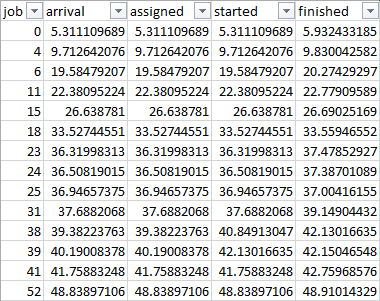
\includegraphics[width=\textwidth]{img/pcg_msa}
        \caption{Simulation run with \gls{msa}}
        \label{fig:pcg_msa}
    \end{minipage}
    \hfill
    \begin{minipage}[b]{0.45\textwidth}
        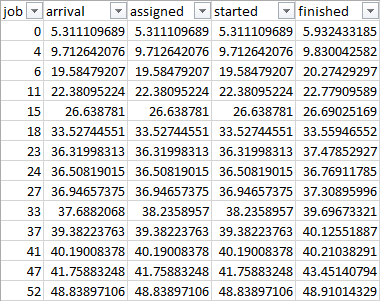
\includegraphics[width=\textwidth]{img/pcg_st}
        \caption{Simulation run with \gls{st}}
        \label{fig:pcg_st}
    \end{minipage}
\end{figure}

\figref{fig:pcg_msa} and \figref{fig:pcg_st} are snippets of the statistical data dumps for two arbitrary simulation runs that clearly display the randomness consistency concept outlined before. When comparing the arrival column on both figures, it is possible to see that even though different number of jobs are being generated, they are consistently generated across different simulation, each arriving at the same simulation time $t$. Note that both figures only show data filtered corresponding to the first direct user task connected to the start event. 

\subsection{User Task}
\label{subsec:user_task}

User task objects also require a simulation environment, a policy, a descriptive name, a service interval and task variability. Each user task has a unique \texttt{child} field which is being set prior to starting the simulation.

Each user task object has a claim token method, which takes tokens as input parameters and finally makes a call to its designed policy, passing the token. On this top level, without stepping into the single policies implementations, the logic is straightforward: start events generate tokens, user tasks that are direct children of start events claim the newly generated tokens, ask the designated policies to assign a user to the token and finally, after a service interval timeout which corresponds to the user's specific service interval has passed, they release the token. The logic can be seen in \lstref{lst:user_task}.

\begin{lstlisting}[caption=User task claim method,label=lst:user_task,style=CustomPython]
    def claim_token(self, token):
        token.worked_by(self)
        policy_job = self.policy.request(self, token)
        service_time = yield policy_job.request_event
        yield self.env.timeout(service_time)
        self.policy.release(policy_job)
\end{lstlisting}

\subsection{Gateway}

Gateways are those process nodes where conditions are tested (see \secref{sec:wfms}). As previously mentioned, in the discrete event simulation environment each newly generated token holds an array with all conditions assigned to it, which are then tested at decision nodes in order to correctly forward or split the token along the path flow. For the purpose of this thesis two types of gateways have been implemented:
\begin{enumerate*}
     \item \gls{xor}
     \item \gls{or} whose logic has been split between its converging and diverging part.
 \end{enumerate*} 

\subsubsection{\glsentryshort{xor}}

\gls{xor}'s logic is straightforward: each gateway has a forward method which is used to correctly move the token along the process. As soon as a token reaches a \gls{xor} gateway, it tests the token's condition and then forwards the token to the next element. The implementation can be seen in \lstref{lst:xor_forward}. Each token holds the 

\begin{lstlisting}[caption=\glsentryshort{xor}'s forward method,label=lst:xor_forward,style=CustomPython]
class XOR(Node):
    def forward(self, token):
        token.worked_by(self)
        action = token.get_action(self)
        child = self.children[action]
        self.child_forward(child, self.env, token)
\end{lstlisting}

\subsubsection{\glsentryshort{or}}

\gls{or} gateways, in contrast to \gls{xor} gateways, require a synchronization between number of split path flows being fired at their diverging state which eventually reach a converging state. In other words, the number of parallel tokens fired at the diverging node must all be accounted for at the converging node. This is achieved by a counter object that each token holds: when a token reaches a divergent \gls{or} gateway, it reads the tokens conditions corresponding to it and for each path flow that the token has to follow it increments the token's counter by $1$. The logic is depicted in \lstref{lst:or_counter_increment}.

\begin{lstlisting}[caption=Token's counter increment logic at a divergent \glsentryshort{or} gateway,label=lst:or_counter_increment,style=CustomPython]
class DOR(Node):
    def choose_child(self, action, token):
        child = self.children[action]
        token.counter.increment()
        self.child_forward(child, self.env, token)
\end{lstlisting}

Each diverging \gls{or} gateway has a corresponding converging \gls{or} gateway which is used to catch all parallel tokens fired by the former. When a token reaches a converging \gls{or} gateway, its counter is decremented each time by $1$ and only when the counter reaches $0$ the token is actually forwarded along. This logic can be seen in \lstref{lst:or_counter_decrement}.

\begin{lstlisting}[caption=Token's counter decrement logic at a convergent \glsentryshort{or} gateway,label=lst:or_counter_decrement,style=CustomPython]
class COR(Node):
    def forward(self, token):
        token.worked_by(self)
        token.counter.decrement()
        if token.counter.count == 0:
            action = token.get_action(self)
            child = self.children[action]
            self.child_forward(child, self.env, token)
\end{lstlisting}

\subsection{End Event}

In \texttt{Python} one does not have to preallocate or deallocate memory by hand as when using pointer based programming languages such as \texttt{C} or \texttt{C++} since this is being taken care of internally. According to \citet{Silver2011}'s definition of activities, processes and end events (refer to \secref{sec:wfms}), when a token reaches an end event, the corresponding process' activity instance is deleted and to be never again used. This is exactly what can be implicitly achieved by \texttt{Python}'s internal garbage collection strategies: tokens are objects that are being generated by start events, when they reach the last element in the process, all references to the token object are extinguished thus effectively engaging the internal garbage collection strategies which deallocate any memory allocation reserved for a token.

\section{Policy Based Role Resolution Implementation}
\label{sec:policy_implementation}
Role resolution according to policies acting as supervisors (as explained in \secref{sec:role_resolution_theory}) in the discrete event simulation environment is achieved by means of a particular class of objects \ie policies and policy jobs.

Policies are a particular object that does not directly participate in the workflow processes, it serves a role as a general supervisor that has the whole overview of the process allowing it to operate on an abstract level. 

The implementation of the policy objects can be seen in \figref{fig:policies_init}.

\fig[0.33\textwidth]{policies_init}{Policies abstract implementation}{fig:policies_init}

Each policy is a blueprint for the actual implementation of the policy itself. It holds minimal information such as a simulation environment, number of users and worker variability.

As a blueprint, each policy object defines two abstract methods for requesting an optimal assignment for a specific token and for later releasing that token and effectively freeing the user that was busy working on it. Refer to \figref{fig:policy_met_att} for its implementation overview.

\fig[0.5\textwidth]{policy_met_att}{Policy methods and attributes}{fig:policy_met_att}

In its request method, each policy generates a policy job object, which is again an abstract implementation of a job that the policy will work in order to return an optimized assignment to a user task. Each policy job requires a user task and a token object as initialization parameters in order to be uniquely identifiable inside the whole process. Moreover, each policy job object serves as a bookkeeping agent by storing and dumping useful information every time its status changes, such as arrival, assigned, started and finished times, assigned user and a list of service times for all available users. Refer to \figref{fig:policyjob_met_att} for its implementation overview.

\fig[0.5\textwidth]{policyjob_met_att}{Policy job methods and attributes}{fig:policyjob_met_att}

In regards to parameters service interval and task variability defined in \subsecref{subsec:user_task} a detailed explanation is required. Both are used to randomly sample service rate intervals for each user active during the simulation. \citet[p. 8]{Zeng2005} in their work follow a two way process to generate such intervals. However in this thesis' implementation a refined version of this process is used:
\begin{enumerate*}
	\item At initialization time, each user task receives a service rate $s$ and a task variability $t$ value
	\item Inside the policy request method, for each user task a sample of an average processing time following an Erlang distribution (a special case of the gamma distribution as defined by \citet{Adan2015}) which takes as input parameters a shape $k$ and a scale $\theta$ is made. The shape value $k$, as the name suggests, defines the curve shape that the Erlang distribution will follow. In this case both values $k$ and $\theta$ are dynamically evaluated at runtime as $k=s/t$ and $\theta = t$. This concept is depicted in \lstref{lst:user_service_rate}
	\item The average processing time becomes a unique value of each user task object and is used by each policy to sample each user's service time, again from an Erlang sampled pool as depicted in \lstref{lst:user_service_rate} and we shall call this value $p_j$.
\end{enumerate*}

For each user eligible to work the assigned token, its service rate is sampled following the Erlang distribution. This time, the Erlang distribution takes as parameters the unique average processing time $p_j$ of user task $j$ and a value worker variability, which is a unique property of each policy, which we shall call $w$.

In order to sample a service rate $p_{ij}$ following the Erlang distribution for each user $i$, shape $k$ is evaluated as $k=p_j/w$ and scale as $\theta = w$ as it can be seen in \lstref{lst:user_service_rate}

\begin{lstlisting}[caption=User service rate sampling following an Erlang distribution,label=lst:user_service_rate,style=CustomPython]
    def request(self, user_task,token):
        average_processing_time = token.random_state.gamma(
            user_task.service_interval ** 2 / user_task.task_variability,
            user_task.task_variability / user_task.service_interval)

        policy_job.service_rate = [token.random_state.gamma(average_processing_time ** 2 / self.worker_variability,
                                                           self.worker_variability / average_processing_time) for
                                   _ in range(self.number_of_users)]
\end{lstlisting}

As previously mentioned, the Erlang distribution is a special case of the Gamma distribution where $k$ defines the shape of the curve. This distribution is better suited to model service rates since with an appropriate $k$ one can approximate a normal distribution without incurring in the aspect of having to manually reset negative values to one (thus loosing statistical generality). This is asserted by the formal definition of Erlang's support with $x \in [0,\infty)$.

\texttt{NumPy}'s implementation of its Erlang distribution is used\foot{https://docs.scipy.org/doc/numpy/reference/generated/numpy.random.gamma.html}{06.01.2017}. \equref{eq:erlang_density} defines the probability density function of the Erlang's distribution with the alternative parametrization that uses $\mu$ instead of $\lambda$ as scale parameter, which is its reciprocal.

\begin{equation}
\label{eq:erlang_density}
	f(x;k,\mu) = \frac{x^{k-1} e^{-\frac{x}{\mu}}}{\mu^k (k-1)!} \text{ for } x,\mu \geq 0
\end{equation}